
%%%%%%%%%%%%%%%%%%%%%%% file typeinst.tex %%%%%%%%%%%%%%%%%%%%%%%%%
%
% This is the LaTeX source for the instructions to authors using
% the LaTeX document class 'llncs.cls' for contributions to
% the Lecture Notes in Computer Sciences series.
% http://www.springer.com/lncs       Springer Heidelberg 2006/05/04
%
% It may be used as a template for your own input - copy it
% to a new file with a new name and use it as the basis
% for your article.
%
% NB: the document class 'llncs' has its own and detailed documentation, see
% ftp://ftp.springer.de/data/pubftp/pub/tex/latex/llncs/latex2e/llncsdoc.pdf
%
%%%%%%%%%%%%%%%%%%%%%%%%%%%%%%%%%%%%%%%%%%%%%%%%%%%%%%%%%%%%%%%%%%%


\documentclass[runningheads,a4paper]{llncs}

\usepackage{amssymb}
\setcounter{tocdepth}{3}
\usepackage{graphicx}


\usepackage{amsmath}

\usepackage{url}
\urldef{\mailsa}\path|{luiza.orosanu, denis.jouvet}@loria.fr|

\newcommand{\keywords}[1]{\par\addvspace\baselineskip
\noindent\keywordname\enspace\ignorespaces#1}

\begin{document}

\mainmatter  % start of an individual contribution

\title{Combining lexical and prosodic features\\for automatic detection of sentence modality\\ in French}
\titlerunning{Automatic detection of sentence modality in French}

\author{Luiza Orosanu$^{1,2,3}$ \and Denis Jouvet$^{1,2,3}$%
%\thanks{The work presented in this article is part of the RAPSODIE project, and has received support from the "Conseil Régional de Lorraine" and from the "Région Lorraine" (FEDER) (http://erocca.com/rapsodie).}
}

\authorrunning{Luiza Orosanu, Denis Jouvet}

\institute{
$^1$ Speech Group, Inria, LORIA, Villers-l\`{e}s-Nancy, F-54600, France \\
$^2$ Universit\'{e} de Lorraine, LORIA, UMR 7503, Villers-l\`{e}s-Nancy, F-54600, France \\
$^3$ CNRS, LORIA, UMR 7503, Villers-l\`{e}s-Nancy, F-54600, France \\
\mailsa\\
\url{}
}


\toctitle{}
\tocauthor{}
\maketitle


\begin{abstract}
This article analyzes the automatic detection of sentence modality in French using both prosodic and linguistic information.
The goal is to later use such an approach as a support for helping communication with deaf people.
Two sentence modalities are evaluated: questions and statements.
As linguistic features, we considered the presence of discriminative interrogative patterns and two log-likelihood ratios of the sentence being a question rather than a statement: one based on words and the other one based on part-of-speech tags.
The prosodic features are based on duration, energy and pitch features estimated over the last prosodic group of the sentence.
The evaluations consider using linguistic features stemming from manual transcriptions or from an automatic speech transcription system.
The behavior of various sets of features are analyzed and compared.
The combination of linguistic and prosodic features gives a slight improvement on automatic transcriptions, where the correct classification performance reaches 72\%.
\keywords{speech-to-text transcriptions, question detection, prosody, likelihood ratio, part-of-speech tags}
\end{abstract}


%%%%%%%%%%%%%%%%%%%%%%%%%%%%%%%%%%%%%%%%%%%%%%%%%%%%%%%%%%%%%%%%%%%%%%%%%%%%%%%%%%%%%%%%%%%%%%%%%%%%%%%%%%%%%%%%%%%%%%%%%%%

\section{Introduction}

The automatic detection of sentence modality has been studied in the past decades with different objectives: to model and detect the speech structure \cite{Jurafsky:1997}, to distinguish questions from statements  \cite{Kral:2005,Yuan:2005,Quang:2006,Quang:2007,Khan:2010,Margolis:2011}, to create the summary of documents or meetings \cite{Quang:2006}, to enrich an automatic transcription with punctuation marks \cite{Kolar:2012}, etc.

The most useful cues for the detection of sentence modality are the prosodic features (computed over the speech signal) and the linguistic features (computed over the word transcription).
There are two scenarios for the linguistic features: when they are extracted from correct data (textual and/or manual transcriptions of audio) or from automatic transcriptions (generated by a speech recognition system). The studies related to automatic speech recognition systems have to additionally take into account the speech recognition errors which get more frequent for poor sound qualities and on spontaneous speech, and can highly decrease the classification performance.

Regarding the prosodic features, different studies on different languages consider different features computed over different parts of the speech signal.
In \cite{Kral:2005}, the prosodic features (pitch and energy) computed on the last 700 milliseconds of speech were used for the detection of French questions.
In \cite{Khan:2010}, the energy and the fundamental frequency were the key features in the detection of Arabic questions.
In \cite{Liscombe:2006} the English question asking behavior was designed in order to improve the intelligent tutoring systems; their study concluded that the most useful features were the pitch slope of the last 200 milliseconds of a turn.
Another detector of French questions (versus statements) made use of 12 prosodic features derived from the fundamental frequency of the entire utterance \cite{Quang:2006}.

When dealing with correct data (e.g. manual transcriptions), considering both prosodic and lexical features proves very useful.
In \cite{Quang:2007}, the combined prosodic-lexical classifier considers lexical features relative to interrogative terms: the unigrams/bigrams preceding or succeeding interrogative terms and the presence (or absence) of interrogative terms.
The use of web textual conversations to detect questions in conversational speech was analyzed in \cite{Margolis:2011}.
Their lexical features consider the presence or absence of unigrams through trigrams in the sentences (with respect to questions or statements).

When dealing with automatic transcriptions, the sentence modality detection becomes more challenging.
In \cite{Jurafsky:1997}, 42 dialog acts were used to model and detect the discourse structure of natural English speech (human-to-human telephone conversations). They used three different types of information (linguistic, prosodic and a statistical discourse grammar) and achieved an accuracy of 65\% on ASR transcripts versus 72\% on reference manual transcripts. Combining recognized words with the discourse grammar was the most useful for this task.
The detection of questions in English meetings was addressed in \cite{Boakye:2009}, using lexico-syntactic, turn related and pitch related information. They achieved an accuracy of 54\% on ASR transcripts versus 70\% on reference manual transcripts. The lexico-syntactic features were the most useful for this task.
The automatic punctuation (comma, period, question mark) of French and English speech-to-text data was studied in \cite{Kolar:2012}. Their boosting-based model uses linguistic (based on word n-grams) and prosodic information and was tested under real world conditions.

Based on the state of the art of question detection, we apply multiple feature combinations on our French data.
Several approaches are analyzed: creating a classifier with only prosodic features or one with only linguistic features or one that combines both linguistic and prosodic
features. Moreover classifier evaluations are carried out using linguistic features stemming out, on the one hand, from manual transcriptions, and on the other hand, from automatic speech-to-text transcriptions.

The work presented in this paper is part of the RAPSODIE project which aims at studying, deepening and enriching the extraction of relevant speech information, in order to support communication with deaf or hard of hearing people.
The detection of sentence modality (questions versus statements) is therefore a key problem here, the deaf or hard of hearing people must be informed when a question
is directed to them, as they should respond or ask for further clarifications.

The paper is organized as follows: section 2 is devoted to the description of the data and tools used in our experiments, section 3 provides a description of the features used for question detection, and section 4 analyzes the results.

%%%%%%%%%%%%%%%%%%%%%%%%%%%%%%%%%%%%%%%%%%%%%%%%%%%%%%%%%%%%%%%%%%%%%%%%%%%%%%%%%%%%%%%%%%%%%%%%%%%%%%%%%%%%%%%%%%%%%%%%%%%
\section{Experimental setup}


%%%%%%%%%%%%%%%%%%%%%%%%%%%%%%%%%%%%%%%%%%%%%%%
\subsection{Textual data for training language models}

Textual punctuated data is used for modeling the lexical and syntactic characteristics of questions and statements.
The available data corresponds to more than 800 million words from the French Gigaword corpus \cite{Mendonca:2011}.
Based on a vocabulary of 97K words, 89K questions and 16M statements were extracted from this corpus by filtering the sentences ending with a question mark, respectively with a dot.
The lexical data was also annotated with part-of-speech (POS) tags; this provided the syntactic data.

Based on the lexical (word-based) data we learned two language models, one for questions and one for statements, with a shared lexicon of 97K words. These language models have the purpose of representing the main word sequences that occur in a question rather than a statement (like for example in French: ``est-ce que ...", ``qu'est-ce que ...", etc).

Based on the syntactic (POS-based) data we learned two other language models, one for questions and one for statements, with a shared lexicon of 36 POS tags. These language models have the purpose of representing the main syntactic sequences that occur in a question rather than a statement (like for example in French the verb-pronoun inversions: ``regardez vous ...", ``pourrait on ...", ``fallait il ...", etc).

Table \ref{Tab:LMs} describes the resulting 3-gram language models based on questions and statements, when using word-based sentences or POS-based sentences.

\begin{table}
\caption{Number of 3-grams in the language models computed over questions and statements}
\label{Tab:LMs}
\centering
\begin{tabular}{|r|r|r|}
\hline
{\bf Language model}  & word-based  & POS-based 	\\ \hline
questions     & 718K  &  9K  	\\ \hline
statements    &  68M  & 16K   	\\ \hline
\end{tabular}
\end{table}


%%%%%%%%%%%%%%%%%%%%%%%%%%%%%%%%%%%%%%%%%%%%%%%
\subsection{Speech and textual data for modality detection}\label{data}

The speech corpora used to train and evaluate the modality detection classifiers (questions versus statements)  come from the ESTER2 \cite{Galliano:2009} and ETAPE \cite{gravier:2012} evaluation campaigns, and from the EPAC \cite{ESTEVE:2010} project.
The ESTER2 and EPAC data are French broadcast news collected from various radio channels (prepared speech and interviews).
The ETAPE data correspond to debates collected from various radio and TV channels (spontaneous speech).
These corpora were manually transcribed and punctuated (the segmentation of speech into sentences is therefore already given).

The set of questions and statements were extracted from these corpora by filtering the sentences ending with a question mark and respectively with a dot.
The training sets of ESTER2, EPAC and ETAPE corpora are used to train the question detection classifiers; the development and test sets of the ESTER2 and ETAPE corpora are used to evaluate them.

The speech training data set contains 10K questions and 98K statements.
However, binary classifiers do not work well when trained with imbalanced data sets: new instances are likely to be classified as the class that has more training samples.
In order to avoid this overfitting problem, we chose to resample the data set by keeping all questions and randomly extracting subsets of statements of the same size (ten different training data sets are considered based on the different random lists of statements).
In the 'Experiments and results' section we present only the average performance (with the associated standard deviation) over all ten training data sets.

Table \ref{Tab:usedData} gives more details on the number of questions and statements used in our experiments.

\begin{table}
\caption{Description of the data used in our experiments }
\label{Tab:usedData}
\centering
\begin{tabular}{|c|r|r|}
\hline
{\bf Data}  & {\bf \# questions}  & {\bf \# statements} 	\\ \hline%\hline
Training data 	& 10077 & 10077  \\ \hline
Evaluation data &   831 &  7005  \\ \hline
\end{tabular}
\end{table}



%%%%%%%%%%%%%%%%%%%%%%%%%%%%%%%%%%%%%%%%%%%%%%%
\subsection{Configuration}

The SRILM tools \cite{Stolcke:2002} were used to train the statistical language models.
The TreeTagger software \cite{Schmid:1994} was used to annotate the transcriptions with POS tags.

The WEKA software \cite{Hall:2009} was used to train and evaluate 5 question detection classifiers:
\begin{itemize}
\item logistic regression (LR) \cite{leCessie:1992},
\item C4.5 decision tree (J48) \cite{Quinlan:1993},
\item rule learner (JRip - Repeated Incremental Pruning to Produce Error Reduction) \cite{Cohen:1995},
\item sequential minimal optimization algorithm for training a support vector classifier (SMO) \cite{Keerthi:2001},
\item neural network using backpropagation to classify instances (MP - Multilayer Perceptron) \cite{Ruck:1990}.
\end{itemize}

The values of F0 in semitones and of the energy are computed every 10 ms from the speech signal using the ETSI/AURORA acoustic analysis \cite{ETSI:2005}.

The forced speech-text alignment is carried out with the Sphinx3 tools \cite{Placeway:1996}. This provides the speech segmentation into phones and words, which is then used to compute the sound durations, as well as to obtain the location and the duration of pauses. As the speech signal quality is rather good, it can be assumed that the segmentation is obtained without major problems.

The pronunciation variants were extracted from the BDLEX lexicon \cite{Calmes:1998} and from in-house pronunciation lexicons, when available.
For the missing words, the pronunciation variants were automatically obtained using JMM-based and CRFbased Grapheme-to-Phoneme converters \cite{Jouvet:2012}.

The Sphinx3 tools were also used to train the phonetic acoustic models and to decode the audio signals.
More information on the large-vocabulary decoding system used in our experiments and its associated lexicon can be found in \cite{Jouvet:2013-1,Jouvet:2013-2}.


%%%%%%%%%%%%%%%%%%%%%%%%%%%%%%%%%%%%%%%%%%%%%%%%%%%%%%%%%%%%%%%%%%%%%%%%%%%%%%%%%%%%%%%%%%%%%%%%%%%%%%%%%%%%%%%%%%%%%%%%%%%
\section{Features for question detection}

%%%%%%%%%%%%%%%%%%%%%%%%%%%%%%%%%%%%%%%%%%%%%%%
\subsection{Linguistic features}

Three linguistic features were used to distinguish questions from statements:

\begin{itemize}
\item Two log-likelihood ratios ({\it lexLLR, synLLR})
\end{itemize}

Two of our linguistic features are represented by the difference between the log-likelihood of the sentence with respect to the 'question' language model and the log-likelihood of the sentence with respect to the 'statement' language model (as done in \cite{Yuan:2005} for Chinese). Computed as:


\begin{equation}
\text{LLR(sentence)}=\text{Log}\left(\frac{\text{P(sentence} \rvert \text{questionLM)}}{\text{P(sentence} \rvert \text{statementLM)}}\right)
\end{equation}

A sentence having a positive {\it LLR} value is likely to be a question. And vice-versa, a sentence having a negative {\it LLR} value is likely to be a statement.

To compute the lexical log-likelihood ratio ({\it lexLLR}) of a sentence we apply the lexical language models (of questions and statements) on its sequence of words.

To compute the syntactic log-likelihood ratio ({\it synLLR}) of a sentence we apply the syntactic language models (of questions and statements) on its sequence of POS tags.


\begin{itemize}
\item Presence of discriminative interrogative patterns ({\it iP})
\end{itemize}

This feature indicates the presence (1) or absence (0) of some discriminative interrogative words or expressions. A sentence having an interrogative pattern is likely to be a question.

A list of sequential patterns was thus extracted from the Gigaword questions transcript with a modified version of the PrefixSpan software \cite{Pei:2001} that considers only consecutive patterns.
Their frequencies were then compared between the Gigaword questions and statements transcripts: those with similar frequencies were removed. The patterns with no interrogative meaning were also removed.

The final list of discriminative interrogative patterns is:
      \{quel, quelle, quels, quelles,
	comment, combien, pourquoi,
	est ce que, est ce qu', qu' est ce, qu' est ce que, qu' est ce qu'\}, corresponding to \{what, which, how, how much, why, ...\}.



%%%%%%%%%%%%%%%%%%%%%%%%%%%%%%%%%%%%%%%%%%%%%%%
\subsection{Prosodic features}

The prosodic features include duration, energy and pitch belonging to the last prosodic group of the sentence.
Prosodic groups are determined according to linguistic information (for grouping grammatical words with corresponding lexical words) and further processing that relies on prosodic information as described in \cite{Bartkova:2013}.
Ten prosodic features were considered in order to distinguish questions from statements. Five are associated to the last syllable of the sentence, and five other are computed on the ending part of the sentence.

The duration of the last vowel is computed from the phonetic segmentation that results from the forced alignment. Its energy corresponds to the mean value calculated over all the frames of the vowel segment. The vowel energy and the vowel duration are then normalized with respect to local mean values computed on non-stressed vowels of the current breath group (speech segment delimited by pauses). In practice we used the vowels that are not in a word final position.
The F0 slope is calculated by linear regression on the speech frames corresponding to the vowel. In addition to the slope, we calculate also, for the vowel, the delta of F0 movement with respect to the preceding vowel. The fifth parameter is the product of the F0 slope by the square of the vowel duration (this is inspired from the glissando threshold).
Other, more global, prosodic parameters are computed on the longest F0 slope that ends in the last syllable of the sentence.  Starting from the last syllable, we go back in time up to detecting an inversion of the F0 slope. We then compute parameters on this longest final F0 slope: the F0 slope itself (determined by linear regression), the length of this longest slope, the total F0 variation between the beginning and the end of the slope, and also the product of the slope by the square of the duration. One last prosodic parameter is used, which corresponds to the F0 level at the end of the sentence, expressed as the percentage of the speaker F0 range (0 corresponding to the lowest F0 value for the speaker, 100 corresponding to the highest F0 value for the speaker).

%%%%%%%%%%%%%%%%%%%%%%%%%%%%%%%%%%%%%%%%%%%%%%%%%%%%%%%%%%%%%%%%%%%%%%%%%%%%%%%%%%%%%%%%%%%%%%%%%%%%%%%%%%%%%%%%%%%%%%%%%%%
\section{Experiments and results}

The classifiers evaluated in our experiments (logistic regression, J48 decision tree, JRip rule learner, SMO sequential minimal optimization algorithm, neural network MP) gave similar results. Thus, only the results obtained with the classifier J48 are presented below.

The classifier evaluations are carried out using features stemming out from:
\begin{itemize}
\item automatic transcriptions (obtained with a large vocabulary speech recognizer) - to study the performance under real conditions
\item manual transcriptions - to study the classifier's maximum performance, obtainable only in ideal conditions (i.e. with perfect transcripts).
\end{itemize}


The performance obtained on our imbalanced test data set (831 questions and 7005 statements) is evaluated by the harmonic mean between the ratio of correctly classified questions and the ratio of correctly classified statements, computed as:

\begin{equation}
\text{H}=\text{2}*\left(\frac{\text{ccQuestions} * \text{ccStatements}}{\text{ccQuestions} + \text{ccStatements}}\right)
\end{equation}

\noindent where ``cc" is an acronym for ``correctly classified".
This value allows us to estimate the global performance of our classifier, given that the performances achieved on questions and on statements are equally important.

\subsection{Prosodic features}

The evaluated combinations of prosodic features are:
\begin{itemize}
\item the last F0 level ($lastF0level$)
\item the 5 features computed over the last syllable ($lastSyl$),
\item the 5 features computed over the last syllable plus the last F0 level ($lastSyl+lastF0level$),
\item the 5 features computed over the ending part of the utterance ($lastPart$),
\item the 6 features related to slope measurements ($slope$),
\item all 10 features ($Prosodic$).
\end{itemize}

\begin{figure}
\begin{center}
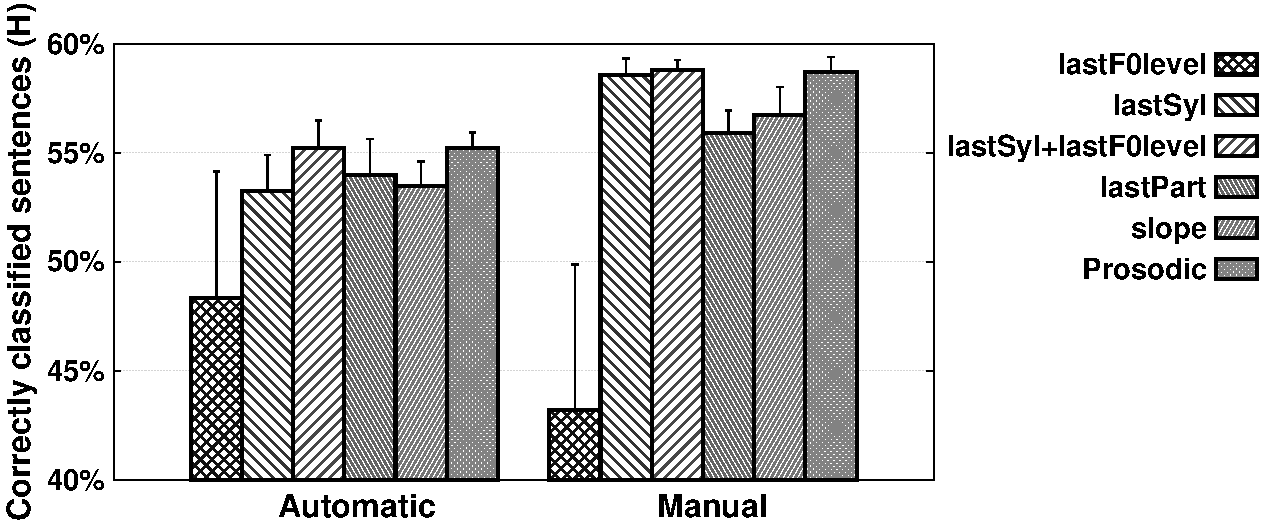
\includegraphics[scale=0.45]{Image/averageStats_compareProsodicFeatures_withSD.pdf}
\end{center}
\caption{Analysis of the average performance obtained when using different prosodic feature combinations on automatic and manual transcriptions}
\label{Fig:P}
\end{figure}



Figure \ref{Fig:P} shows the average performance obtained with different prosodic feature combinations on automatic and manual transcriptions. % and it proves the importance of using and combining all of them.
The most important prosodic features are those computed over the last syllable of the utterance in combination with the last F0 level ($lastSyl+lastF0level$).
Combining all 10 prosodic features ($Prosodic$) does not deteriorate this performance: they are all considered to be useful and kept in the following experiments.
The performance loss between manual and automatic transcriptions (of about 3\%) is due to recognition errors and to the automatic word (phone) segmentation.



\subsection{Linguistic features}

The evaluated combinations of linguistic features are:
\begin{itemize}
\item the lexical log-likelihood ratio ($lexLLR$)
\item the syntactic log-likelihood ratio ($synLLR$),
\item the lexical log-likelihood ratio plus the presence of discriminative interrogative patterns ($lexLLR+iP$),
\item the syntactic log-likelihood ratio plus the presence of discriminative interrogative patterns ($synLLR+iP$),
\item both log-likelihood ratios ($lexLLR+synLLR$),
\item all 3 features ($Linguistic$).
\end{itemize}


\begin{figure}
\begin{center}
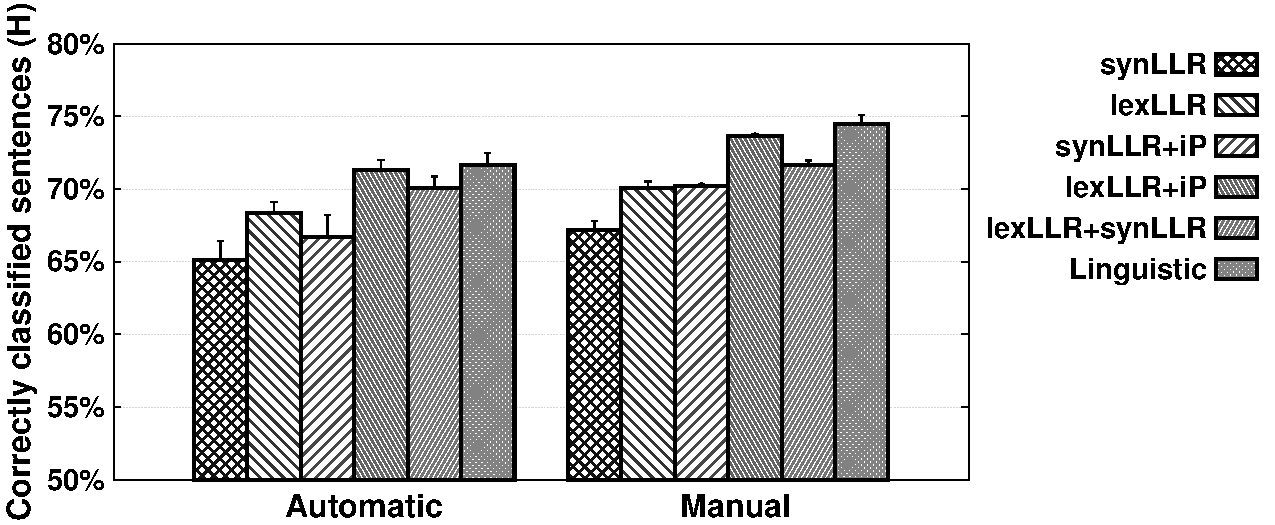
\includegraphics[scale=0.5]{Image/averageStats_compareLinguisticFeatures_withSD.pdf}
\end{center}
\caption{Analysis of the average performance obtained when using different linguistic feature combinations on automatic and manual transcriptions}
\label{Fig:L}
\end{figure}


Figure \ref{Fig:L} shows the average performance obtained with different linguistic feature combinations on automatic and manual transcriptions and it proves the importance of using and combining all of them.
The most important linguistic feature is the lexical log-likelihood ratio ($lexLLR$).
Combining it with the presence of discriminative interrogative patterns ($lexLLR+iP$) is more useful than combining it with the syntactic log-likelihood ratio ($lexLLR+synLLR$).
The performance loss between manual and automatic transcriptions of the combined set of interrogative patterns and syntactic log-likelihood ratio ($synLLR+IP$) is bigger than the one achieved by the $lexLLR$ feature, which means that they are less tolerant to recognition errors.
However, the combination of all three features ($Linguistic$) improves the classification performance, especially when dealing with correct transcriptions.


\subsection{Combined prosodic-linguistic features}

Table \ref{Tab:perfAM} shows the average performance (harmonic mean $H$, along with the ratios of correctly classified questions and  correctly classified statements) obtained with the prosodic, linguistic and combined features, when applied on automatic speech-to-text transcriptions and on manual transcriptions.
It can be easily observed that the linguistic classifiers outperform the prosodic classifiers.
The performance obtained with the linguistic classifiers when applied on the automatic transcriptions and on the manual transcriptions differs by about 3\% absolute, due to recognition errors (22\% word error rate on Ester and 28\% on Etape) and most likely to the misrecognition of the interrogative words.
The combination of linguistic and prosodic features does not provide any improvement on manual transcripts and provides only a slight improvement on automatic transcription.

\begin{table}
\caption{Average performance (harmonic mean $H$, along with the ratios of correctly classified questions and  correctly classified statements respectively) obtained on automatic and manual transcriptions, for prosodic features alone, linguistic features alone and with a combination of prosodic and linguistic features}
\label{Tab:perfAM}
\centering
\begin{tabular}{|p{2.3cm}|p{3cm}|p{3cm}|p{3cm}|}
\hline
{\bf Transcripts}  	& {\bf Prosodic}  		& {\bf Linguistic} 		& {\bf Combined}	\\ \hline
automatic 		& 55.24  (51.71; 60.23)  	& 71.64  (66.62; 77.77) 	& 72.21  (69.55; 75.25)	\\ \hline
manual 			& 58.69  (57.97; 59.55) 	& 74.47  (71.57; 77.93) 	& 74.26	 (75.18; 73.46)	\\ \hline
\end{tabular}
\end{table}

Table \ref{Tab:cMatrix} gives more detailed results obtained with the combined prosodic-linguistic classifier on the manual transcriptions, when trained on a single random training set.
627 out of 831 questions were correctly classified as questions (ccQ=$75.45\%$) and 5047 out of 7005 statements were correctly classified as statements (ccS=$72.05\%$).
The harmonic average performance is here H=$73.71\%$.

\begin{table}
\renewcommand{\arraystretch}{1.3}
\caption{Confusion matrix between questions and statements obtained on manual transcriptions with the combined prosodic-linguistic classifier, when trained on a single random training set}
\label{Tab:cMatrix}
\centering
\begin{tabular}{p{2.01cm}|p{1.8cm}|p{1.8cm}|p{2.5cm}}
\cline{2-3}
& classified as \textbf{Question} & classified as \textbf{Statement} &   \\
\end{tabular}

\begin{tabular}{|p{2cm}|p{1.8cm}|p{1.8cm}|p{2.5cm}}
\cline{1-3}
\textbf{Question}  &    627 & 204   & \textbf{ccQuestions=75.45\%} \\ \cline{1-3}
\textbf{Statement} &  1958 & 5047   & \textbf{ccStatements=72.05\%} \\ \cline{1-3}
\end{tabular}
\end{table}


\subsection{Combined outputs}

A final experiment consisted in combining the outputs of all five classifiers (when using all 13 prosodic-linguistic features).
Each classifier makes a class prediction (question or statement) on each utterance of the test data set.
The final decision is made by a majority vote: if most of the classifiers (in this case at least 3) assign the utterance to class ``question", than the utterance is assigned to class ``question"; if not, than the utterance is assigned to class ``statement".

Table \ref{Tab:mixC} shows the average performance ($H$) obtained with all five classifiers separately, and with their combination (by majority vote).
The majority vote and the 5 classifiers have similar performances, thus confirming that the 5 classifiers are likely to agree on the class predictions.

\begin{table}
\renewcommand{\arraystretch}{1.3}
\caption{Average performance ($H$) obtained with all 5 classifiers and with their combination (by majority vote) on manual and on automatic transcriptions}
\label{Tab:mixC}
\centering
\begin{tabular}{|p{2cm}|p{1.2cm}|p{1.2cm}|p{1.2cm}|p{1.2cm}|p{1.2cm}|p{2cm}|}
\cline{2-7}
\multicolumn{1}{c|}{}	& LR		& J48		& JRip		& SMO		& MP		& combination 	\\ \hline
\textbf{Automatic}  	& 72.04  	& 72.21		& 72.81		& 69.56		& 72.07		& 72.66		\\ \hline
\textbf{Manual} 	& 73.34 	& 74.26		& 74.12		& 72.09		& 74.33		& 74.91		\\ \hline
\end{tabular}
\end{table}



%%%%%%%%%%%%%%%%%%%%%%%%%%%%%%%%%%%%%%%%%%%%%%%%%%%%%%%%%%%%%%%%%%%%%%%%%%%%%%%%%%%%%%%%%%%%%%%%%%%%%%%%%%%%%%%%%%%%%%%%%%%
\section{Conclusions}

This paper analyzed the impact of linguistic features, prosodic features and combined linguistic-prosodic features when developing an automatic question detector.
The context of this work is to support the communication with deaf or hard of hearing people, which requires an automatic detection of questions in order to inform them when a question is directed to them. The experiments were carried out using three French speech corpora: ETAPE, EPAC and ESTER2.

Different types of classifiers (logistic regression, decision tree, rule learner, sequential minimal optimization algorithm, neural network) were evaluated, but they all give similar results.

The prosodic classifier (based on 10 prosodic features) has a poor performance: it hardly exceeds 55\% of correctly classified sentences.
The most important prosodic features are those computed over the last syllable, in combination with the last F0 level.

The linguistic classifier (based on 3 linguistic features) provides by far better results: 72\% when it is applied on ASR transcriptions (with perfect sentence boundaries) versus 74\% when it is applied on reference manual transcripts. The most important linguistic feature is  the lexical log-likelihood ratio (computed with respect to word-based language models).

The combination of prosodic and linguistic features does not provide any improvement on manual transcripts, but it provides a slight improvement on automatic transcription.

Future work will investigate further prosodic and linguistic features; confidence measures will also be considered in the computation of the linguistic features.

%%%%%%%%%%%%%%%%%%%%%%%%%%%%%%%%%%%%%%%%%%%%%%%%%%%%%%%%%%%%%%%%%%%%%%%%%%%%%%%%%%%%%%%%%%%%%%%%%%%%%%%%%%%%%%%%%%%%%%%%%%%
\subsubsection*{Acknowledgements}

The work presented in this article is part of the RAPSODIE project, and has received
support from the "Conseil R\'{e}gional de Lorraine" and from the "R\'{e}gion Lorraine" (FEDER) (http://erocca.com/rapsodie).


% Bibliography
\bibliographystyle{splncs03}
\bibliography{myBib_QD}


\end{document}
